\chapter{Laboratorio de pruebas}
\label{chapter6}

% **************************** Define Graphics Path **************************
\ifpdf
    \graphicspath{{Chapter6/Figs/Raster/}{Chapter6/Figs/PDF/}{Chapter6/Figs/}}
\else
    \graphicspath{{Chapter6/Figs/Vector/}{Chapter6/Figs/}}
\fi

Para validar funcionalmente el prototipo es preciso la construcción de un laboratorio de experimentación sobre el cual ejecutar un conjunto de pruebas e implementar algunos casos de uso representativos. Dentro de las pruebas funcionales se busca verificar aspectos importantes de la implementaci\'on como la clasificación de tr\'afico, el algoritmo de ruteo dinámico y el algoritmo de distribución de etiquetas. Por otro lado con la implementaci\'on de algunos casos de uso representativos se busca validar la utilización del enfoque OpenFlow/SDN en la construcci\'on de la RAU2.

El siguiente cap\'itulo est\'a destinado a la presentación del laboratorio de pruebas construido y a la descripción de las diferentes pruebas realizadas.

% **************************** Construccion del TestBed ************************** 
\section{Definición del Laboratorio}

Como se menciona anteriormente uno de los objetivos de este laboratorio de experimentación es verificar el correcto funcionamiento de la implementaci\'on realizada, en particular en los aspectos críticos de la misma como la capacidad para clasificar tr\'afico y los diferentes algoritmos de ruteo, distribución de etiquetas, actualización topol\'ogica. 

Para esto es necesario construir un prototipo con suficientes nodos y enlaces como para poder definir varios servicios de redes privadas. Tambi\'en interesa la existencia de caminos alternativos entre un par de nodos origen y destino para poder comprobar el funcionamiento del algoritmo de ruteo y evaluar el comportamiento del prototipo ante cambios en la topolog\'ia (desconexi\'on de nodos o fallas en enlaces por mencionar algunos ejemplos).

Teniendo en cuenta los requerimientos mencionados se construye un laboratorio de pruebas con la siguiente topolog\'ia (ver figura \ref{fig:LaboratorioDePruebasTopo}).
  
\begin{figure}[ht!] 
\centering    
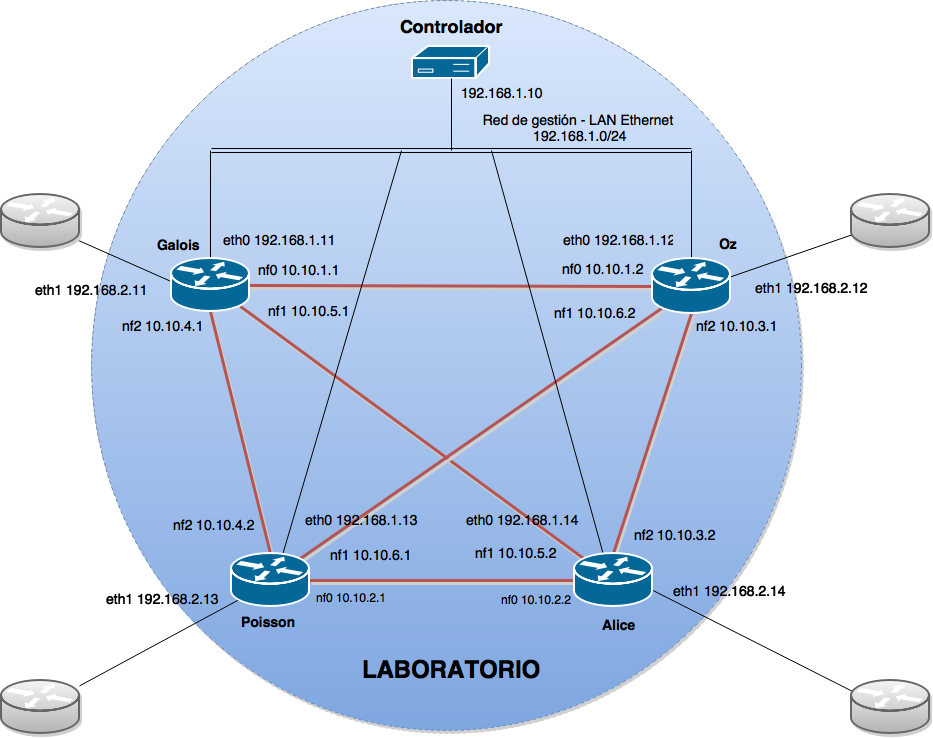
\includegraphics[width=0.7\textwidth]{Topologia}
\caption[Laboratorio de pruebas - Topolog\'ia]{Laboratorio de pruebas - Topolog\'ia}
\label{fig:LaboratorioDePruebasTopo}
\end{figure}

El laboratorio se compone de cuatro nodos implementados en base al dispositivo RAU-Switch conectados entre si con enlaces de fibra \'optica multimodo. Cada nodo est\'a conectado a los otros tres nodos de la topolog\'ia implementando de esta forma una topolog\'ia full mesh de cuatro nodos. A su vez cada nodo est\'a conectado al controlador SDN del prototipo mediante una interfaz de red ethernet (interfaces \textbf{eth0}).

Por la forma que tiene la topolog\'ia, los cuatro nodos nombrados \textit{Galois}, \textit{Poisson}, \textit{Oz} y \textit{Alice} son nodos de borde. Esto quiere decir que RAUFlow los considera como nodos habilitados para ser nodo de ingreso o egreso en la definici\'on de servicios de redes privadas.

Por otro lado cada nodo cuenta con una interfaz de red de ethernet adicional (interfaz \textbf{eth1}) utilizada como interfaz externa para la conexi\'on con otras subredes. Estas interfaces son utilizadas por RAUFlow para la definici\'on de servicios de VPN como los puntos de entrada y salida de tr\'afico. Por tanto cada una de estas interfaces se encuentra directamente conectada a la subred de una VPN en particular.

Como se menciona anteriormente en el cap\'itulo 5, la representaci\'on utilizada para modelar una topolog\'ia de red es la de un multigrafo dirigido ponderado. En la figura \ref{fig:LaboratorioDePruebasCostos} se muestra esta representaci\'on para la topolog\'ia del prototipo. Como puede apreciarse en la imagen cada enlace tiene un costo asociado. Este costo se define mediante el archivo de configuraci\'on del demonio Unix OSPF en cada nodo de la red y es utilizado por el algoritmo SPF centralizado para el c\'alculo de las mejores rutas.

Por simplicidad en el diagrama se han obviado los enlaces existentes entre el Controlador y cada uno de los nodos. Como se menciona en el cap\'itulo 4 la instancia de Quagga ejecutada en el controlador tiene como \'unico objetivo contar con un acceso local a la LSDB. Por ello conceptualmente el costo asociado a cada uno de estos enlaces es infinito, lo cual en la pr\'actica se realiza asignando el valor 65535.  

\begin{figure}[ht!] 
\centering    
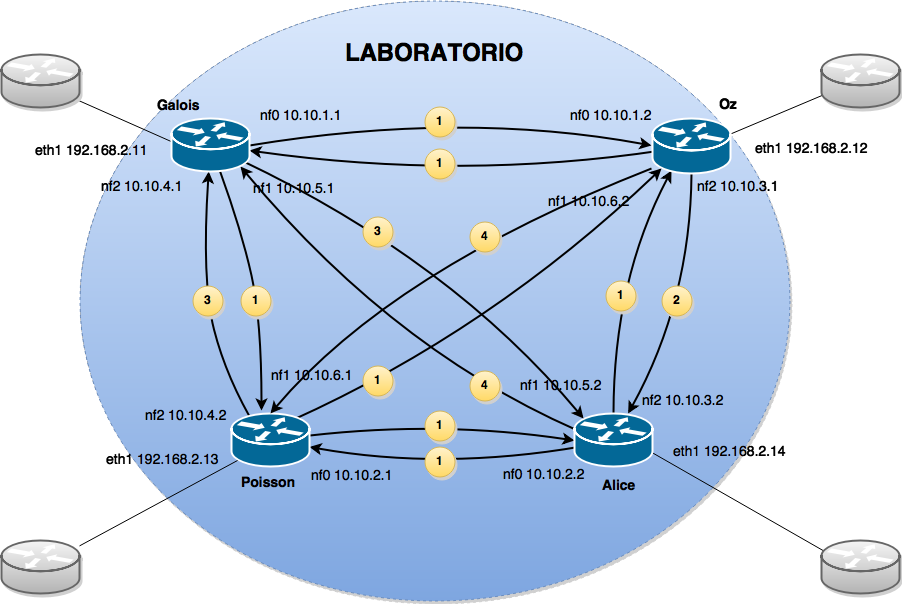
\includegraphics[width=0.70\textwidth]{TopologiaCostos}
\caption[Laboratorio de pruebas - Costos de enlaces en la topolog\'ia]{Laboratorio de pruebas - Costos de enlaces en la topolog\'ia}
\label{fig:LaboratorioDePruebasCostos}
\end{figure}

Sobre este laboratorio se implementan dos casos de uso representativos: (a) VPN de capa 3 y (b) VPN de capa 2. Sobre cada uno de estos casos de uso a su vez se ejecutan una serie de pruebas orientadas a verificar el correcto funcionamiento de las componentes m\'as importantes en la implementaci\'on de RAUFlow y RAU-Switch.

A continuaci\'on se describen los resultados obtenidos en la implementaci\'on de estos casos de uso y la ejecuci\'on de estas pruebas, comenzando por el caso de uso VPN de capa 3.

\section{VPN de capa 3}

Las redes privadas virtuales de capa 3 son un tipo de servicio comúnmente brindado por un operador de red y es uno de los servicios que se quiere implementar en la RAU2. Sobre este tipo de redes privadas puede implementarse clasificaci\'on de tr\'afico por tipo de aplicaci\'on o numeraci\'on de capa 3 por citar algunos ejemplos.

En este trabajo se implementan dos escenarios diferentes para este tipo de red privada: (a) red privada multipunto con una \'unica organizaci\'on y tres sucursales f\'isicamente separadas, (b) red privada punto a punto con dos organizaciones, cada una de ellas con dos sucursales f\'isicamente separadas. 

A continuaci\'on se detalla la construcci\'on de ambos escenarios y los resultados obtenidos.

\subsection{Escenario 1}

Este escenario representa una red privada multipunto de capa 3. En el mismo se tiene una sola organizaci\'on o red privada dividida en 3 sucursales o subredes físicamente separadas.

En el laboratorio cada una de estas subredes y de aqu\'i en m\'as cada subred cliente en los siguientes escenarios de pruebas son implementadas mediante el emulador Core\cite{Core}. Esta herramienta permite emular dispositivos de red como routers, switches y las conexiones entre ellos mediante maquinas virtuales Linux. 

\begin{figure}[ht!] 
\centering    
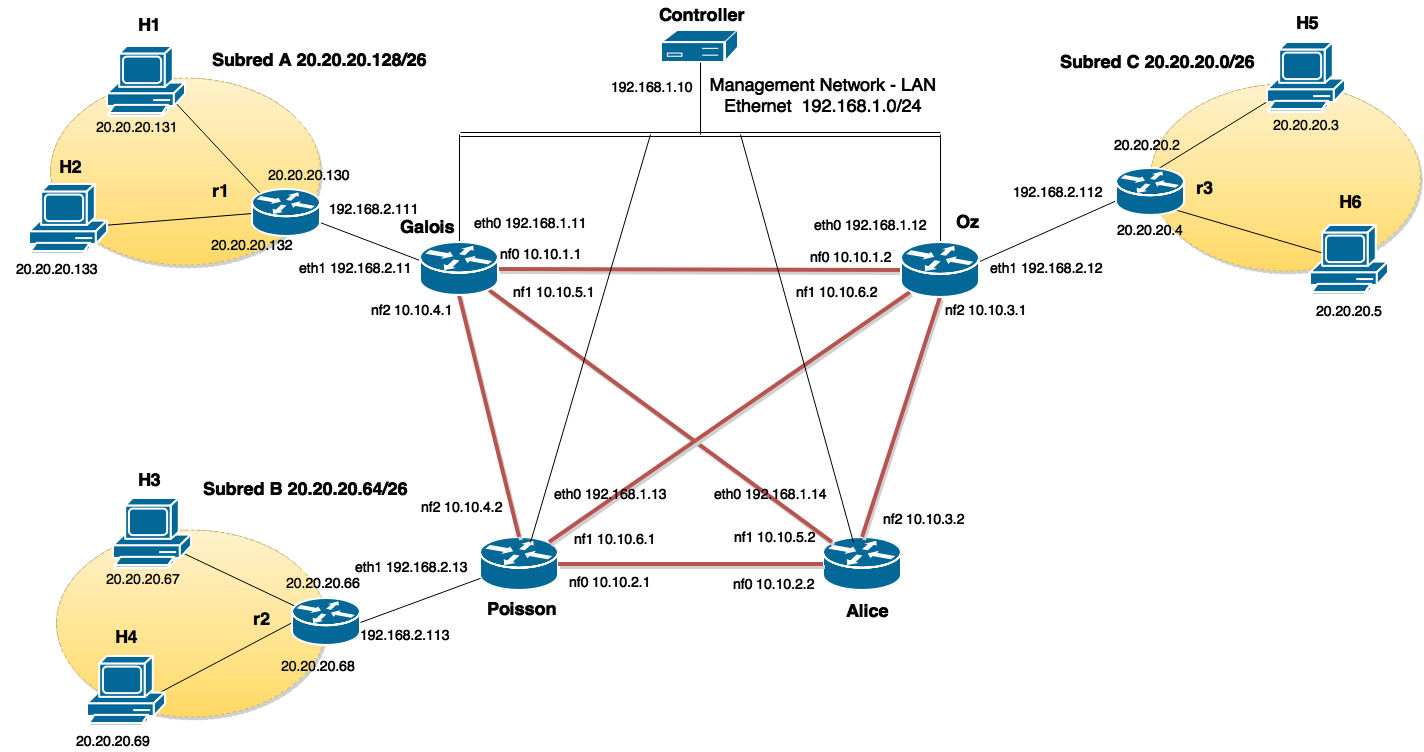
\includegraphics[width=1.0\textwidth]{CU1P1}
\caption[VPN de capa 3 - Escenario 1]{VPN de capa 3 - Escenario 1}
\label{fig:CUP1}
\end{figure}

Sobre este escenario se ejecutan una serie de pruebas orientadas a verificar los siguientes aspectos relacionados al prototipo:

\begin{enumerate}
\item Algoritmo de ruteo
\item Algoritmo de distribución de etiquetas
\item Clasificaci\'on de tr\'afico
\item Actualizaci\'on de rutas cuando cambia la topolog\'ia
\item Capacidad para crear VPN multipunto
\end{enumerate}

Para construir la red privada multipunto uniendo las tres subredes mencionadas y adem\'as verificar los puntos anteriores, se instancia los siguientes servicios (ver tabla \ref{table:TablaFlujos}). Por cada par de subredes se crean dos servicios (un servicio para cada sentido del tr\'afico).

\begin{table}[h]
\begin{tabular}{| l | l | l | p{4cm} | p{4cm} |}
\hline
Nombre & Ingreso & Egreso & Clasificación & Descripción \\ \hline

\crule[Aquamarine]{0.3cm}{0.3cm} S1 & Galois - eth1 & Oz - eth1 & ip\_src=20.20.20.128/26 ip\_dst=20.20.20.0/26 & Tr\'afico IP de Subred A a Subred C \\ \hline

\crule[Red]{0.3cm}{0.3cm} S2 & Oz - eth1 & Galois - eth1 & ip\_src=20.20.20.0/26 ip\_dst=20.20.20.128/26 & Tr\'afico IP de Subred C a Subred A \\ \hline

\crule[ForestGreen]{0.3cm}{0.3cm} S3 & Galois - eth1 & Poisson - eth1 & ip\_src=20.20.20.128/26 ip\_dst=20.20.20.64/26 & Tr\'afico IP de Subred A a Subred B \\ \hline

\crule[LimeGreen]{0.3cm}{0.3cm} S4 & Poisson - eth1 & Galois - eth1 & ip\_src=20.20.20.64/26 ip\_dst=20.20.20.128/26 & Tr\'afico IP de Subred B a Subred A \\ \hline

\crule[RoyalPurple]{0.3cm}{0.3cm} S5 & Poisson - eth1 & Oz - eth1 & ip\_src=20.20.20.64/26 ip\_dst=20.20.20.0/26 & Tr\'afico IP de Subred B a Subred C \\ \hline

\crule[YellowOrange]{0.3cm}{0.3cm} S6 & Oz - eth1 & Poisson - eth1 & ip\_src=20.20.20.0/26 ip\_dst=20.20.20.64/26 & Tr\'afico IP de Subred C a Subred B \\ \hline 

\end{tabular}
\vspace{0.3cm}
\caption[VPN capa 3 - Escenario 1, servicios creados]{VPN capa 3 - Escenario 1, servicios creados}
\label{table:TablaFlujos}
\end{table}

Para cada uno de estos servicios adem\'as se indica el etherype 0x0800 correspondiente al tipo de tr\'afico IPv4.

Este conjunto de servicios establece el procesamiento de paquetes de capa 3 para las diferentes subredes de forma de conectarlas en una red privada de capa 3. A continuaci\'on se detallan las pruebas realizadas para cada uno de los aspectos mencionados anteriormente.

\subsubsection{Verificaci\'on del Algoritmo de ruteo}
En esta secci\'on se eval\'ua el correcto funcionamiento del algoritmo de ruteo. Para ello se comparan los caminos computados por el algoritmo para cada servicio, con los respectivos mejores caminos te\'oricos (previamente calculados de forma manual). 

Para cada camino se verifican dos cosas: (1) que el camino calculado se corresponde con el camino te\'orico y (2) que el camino es correctamente instalado en forma de reglas de reenvío (en base a conmutaci\'on de etiquetas) en las respectivas tablas de flujos OpenFlow de cada nodo del camino.

Como se ha mencionado, los caminos te\'oricos son calculados manualmente observando los costos de la topolog\'ia (figura \ref{fig:LaboratorioDePruebasCostos}). Los resultados de este procedimiento se muestran en la figura \ref{fig:CUP1Caminos}, identificado cada camino mediante el código de colores utilizado en la tabla de servicios.

\begin{figure}[ht!] 
\centering    
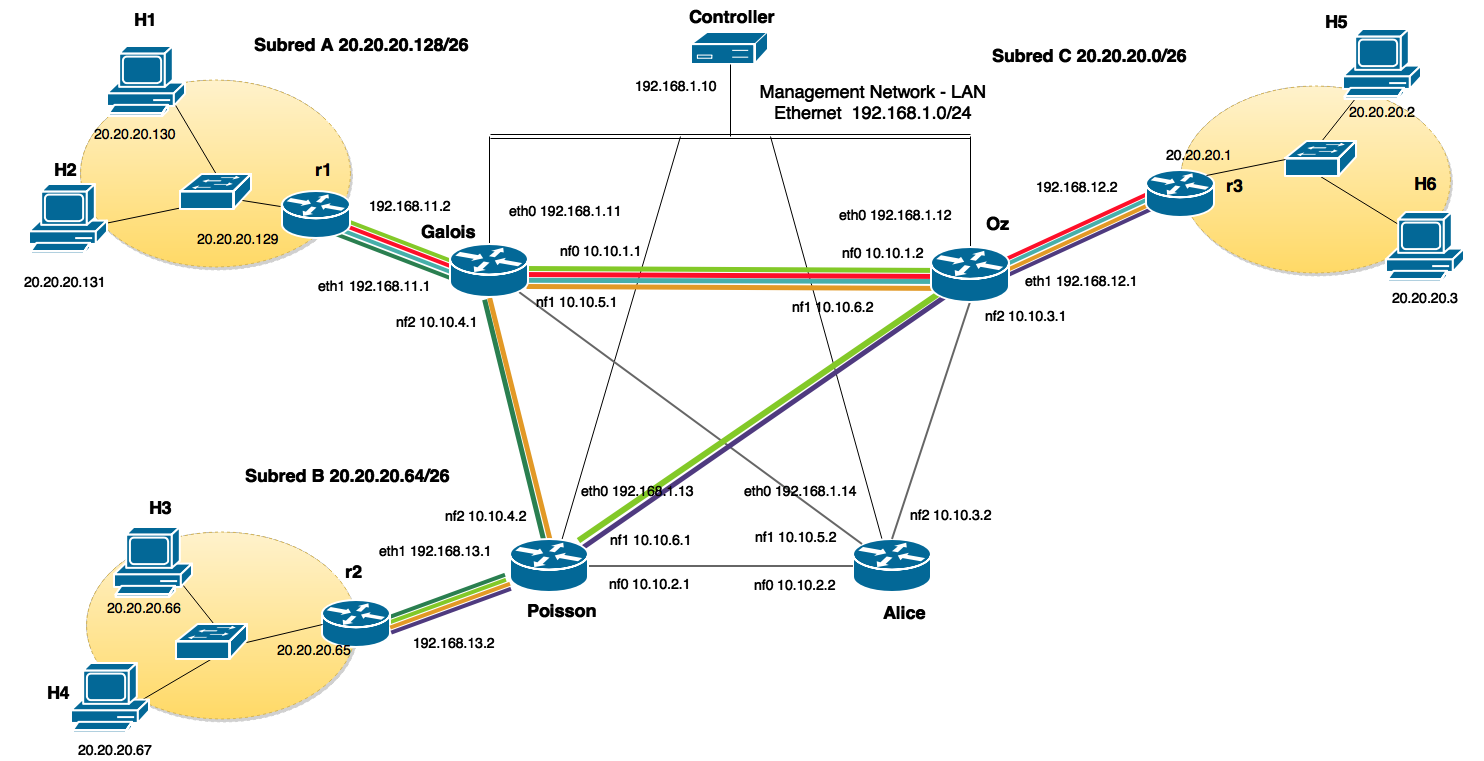
\includegraphics[width=1.0\textwidth]{CU1P1Caminos}
\caption[Escenario 1 - LSPs]{Escenario 1 - LSPs}
\label{fig:CUP1Caminos}
\end{figure}

Para obtener los caminos calculados por el algoritmo de ruteo se analizan las tablas de flujos de Open vSwitch en cada uno de los nodos de la red prototipo utilizando el comando \textbf{dump-flows} de esta herramienta; de esta forma a partir de la informaci\'on en las mismas se construye cada uno de los caminos. Cabe destacar que tambi\'en puede obtenerse la informaci\'on de las tablas de flujos mediante la interfaz gráfica de RAUFlow.

Aplicando este procedimiento para cada uno de los servicios en la tabla \ref{table:TablaFlujos} se comprueba la correspondencia entre los caminos computados por el algoritmo de ruteo y los caminos te\'oricos, a la vez que se comprueba que son correctamente instalados como flujos en las tablas de cada nodo en el prototipo. En el apéndice \ref{appendix6.1} se incluye a modo de ejemplo el análisis realizado para los LSPs asociados a los servicios S3 y S4.
 
\subsubsection{Clasificaci\'on de tr\'afico}
Para cada servicio se implementa clasificaci\'on de tr\'afico en el prototipo solamente en el nodo ingreso, implementándose para el escenario definido en base a la numeraci\'on IP origen y destino de un paquete. Luego en cada nodo intermedio los paquetes son procesados acorde a las reglas de reenvío basadas en la conmutación de etiquetas MPLS.

Para verificar que realmente se implementa clasificaci\'on de tr\'afico se observa el comportamiento de cada flujo OpenFlow involucrado en el procesamiento del tr\'afico asociado a un servicio (flujos que clasifican tr\'afico en el nodo de ingreso y flujos que construyen un LSP). Para ello se genera tr\'afico para los servicios definidos (ver tabla \ref{table:TablaFlujos}) y mediante la herramienta de Linux \textbf{tcpdump} se captura tr\'afico por las diferentes interfaces en cada nodo involucrado en los LSPs correspondientes. 

Mediante este procedimiento se genera tr\'afico para todos los servicios definidos, constatando que el mismo es correctamente enrutado a trav\'es de la red laboratorio mediante flujos OpenFlow y siendo entregado a la respectiva subred destino. Por simplicidad los detalles t\'ecnicos de este procedimiento se han omitido de este cap\'itulo, aunque si el lector desea profundizar en ellos se incluye en el ap\'endice \ref{appendix6.2} una descripci\'on de este procedimiento y los resultados obtenidos para los servicios S1 y S3.

En la siguiente secci\'on se discute el comportamiento del prototipo, cuando la topolog\'ia cambia por ejemplo por una falla t\'ecnica en un enlace, utilizando el escenario y los servicios definidos anteriormente.

\subsubsection{Actualizaci\'on de rutas}
Para probar el correcto funcionamiento del algoritmo de ruteo en la actualizaci\'on de rutas ante un cambio en la topolog\'ia, se trabaja con los servicios previamente definidos en \ref{table:TablaFlujos}. Partiendo de este escenario, se simula un desperfecto t\'ecnico en los enlaces \\ $<(Galois, nf_2), (Poisson, nf_2)>$ y  $<(Poisson, nf_2), (Poisson, nf_2)>$ (por ejemplo desconectando el cable que conecta ambos nodos), provocando de esta forma una actualizaci\'on en la topolog\'ia y la posterior ejecuci\'on de los algoritmos de ruteo y distribución de etiquetas para los nuevos LSPs.
 
Acorde a los costos de la topolog\'ia (ver figura \ref{fig:LaboratorioDePruebasCostos}), en la nueva topolog\'ia los caminos te\'oricos asociados a cada servicio quedan de la siguiente forma:

\begin{figure}[h] 
\centering    
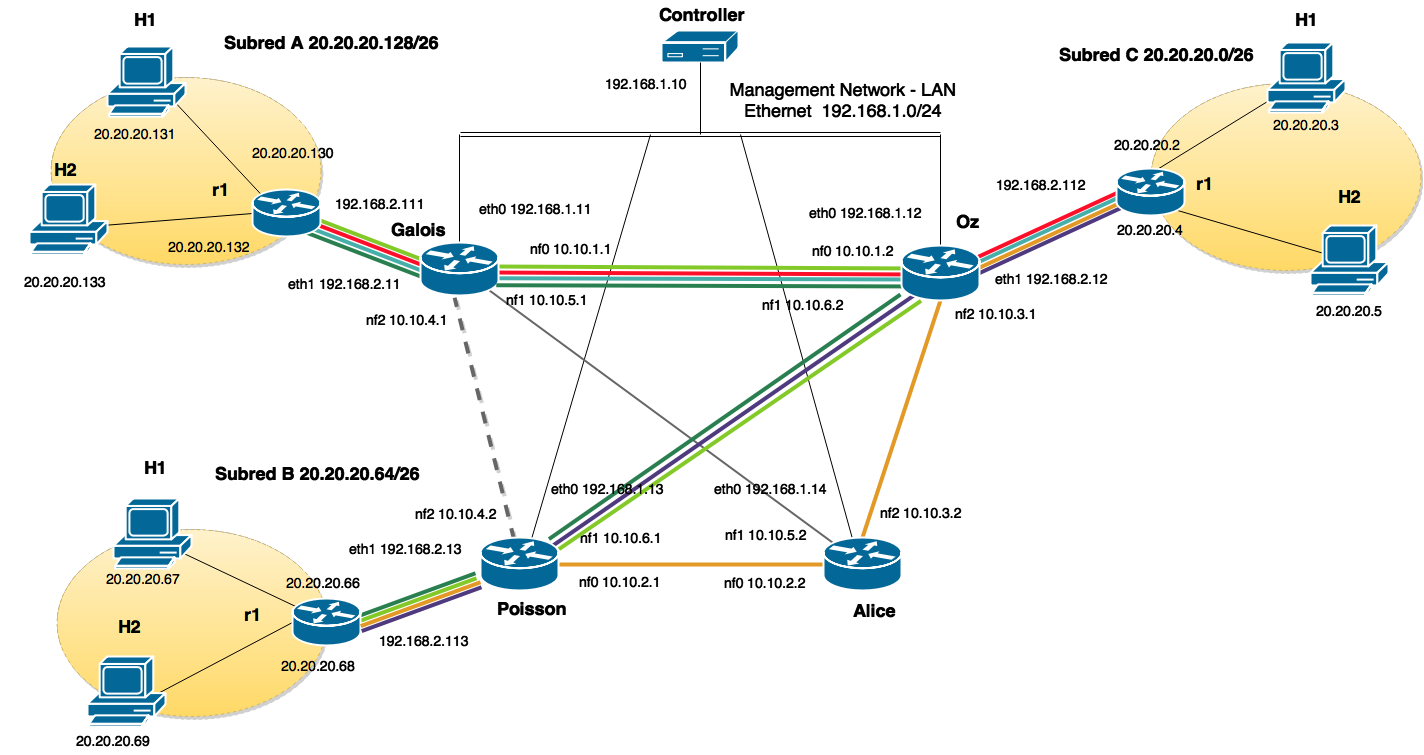
\includegraphics[width=1.0\textwidth]{CU1P1CaminosRecalculo}
\caption[Escenario 1 - Caminos para servicios recalculados]{Escenario 1 - Caminos para servicios recalculados}
\label{fig:CUP1Caminos2}
\end{figure}
 
N\'otese que los \'unicos caminos que cambian son los asociados a los servicios S3 y S6. Cabe destacar adem\'as que en la nueva topolog\'ia existe m\'as de un camino de m\'inimo costo para el servicio S3; los caminos $<(Galois, nf0), (Oz, nf1)>$ y \\ $<(Galois, nf0), (Oz, nf2), (Alice, nf0)>$ presentan ambos el costo 4. Por tanto se tienen dos resultados v\'alidos posibles para la salida del algoritmo de ruteo para este servicio.

Analizando nuevamente las tablas de flujos de cada nodo en el laboratorio, se comparan los caminos computados por el algoritmo de ruteo con los caminos te\'oricos para cada servicio. Mediante este procedimiento se comprueba la correcta actualizaci\'on de caminos LSPs tras un cambio en la topolog\'ia. En el ap\'endice \ref{appendix6.3} se muestran los detalles t\'ecnicos de este procedimiento para los LSPs asociados a los servicios S3 y S6.
 
De esta forma se verifica para el laboratorio de pruebas construido, la correctitud del algoritmo de ruteo, el algoritmo de distribución de etiquetas, se prueba el correcto funcionamiento de las tablas de flujos Open vSwitch y los flujos particulares utilizados para implementar clasificación de tr\'afico, se comprueba el correcto accionar del programa ante cambios en la topolog\'ia (recalculo de LSPs) y finalmente se valida la construcción de un servicio de red privada multipunto de capa 3.

En la siguiente seccci\'on se discute la verificación de otros aspectos importantes en el funcionamiento del prototipo, utilizando como escenario de pruebas la construcci\'on de dos servicios de red privada punto a punto de capa 3, utilizando dos organizaciones diferentes.   

\subsection{Escenario 2}

Este escenario (ver figura \ref{fig:CUP2}) representa una red privada punto a punto de capa 3. Est\'a compuesto por dos organizaciones diferentes, cada una de ellas con dos sucursales f\'isicamente separadas. Adem\'as, ambas organizaciones utilizan el mismo espacio de direcciones IP para sus respectivas subredes.

\begin{figure}[h!] 
\centering    
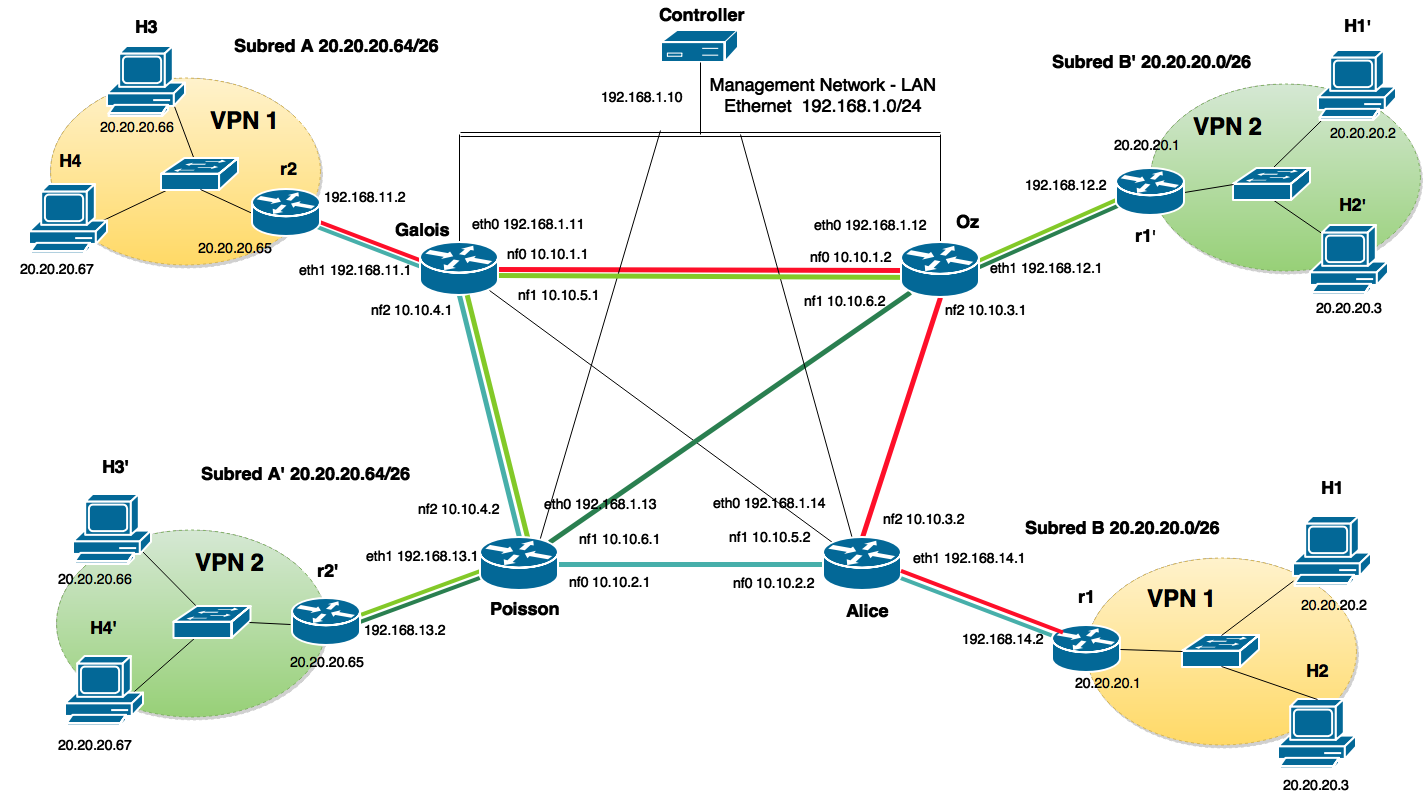
\includegraphics[width=1.0\textwidth]{CU1P2Caminos}
\caption[VPN de capa 3 - Escenario 2]{VPN de capa 3 - Escenario 2}
\label{fig:CUP2}
\end{figure}

Este escenario se traduce en dos servicios de VPN punto a punto, aunque los aspectos de implementaci\'on que en esta secci\'on se pretenden verificar son independientes de si el servicio de VPN es punto a punto o multipunto. Sobre este escenario se busca validar los siguientes aspectos en relaci\'on a la implementaci\'on:

\begin{enumerate}
\item El prototipo soporta la construcci\'on de servicios de VPN de capa 3 para múltiples organizaciones (recordar que en el escenario anterior se trabaja con una \'unica organización).

\item La implementaci\'on utilizada en el prototipo para transportar tr\'afico de una organización desde un nodo de ingreso a un nodo de egreso, es independiente de la numeraci\'on de capa 3 de dicho tr\'afico. En otras palabras soporta organizaciones con numeraci\'on IP solapadas.
\end{enumerate}

Para la construcci\'on de este escenario se instancia los siguientes servicios en el sistema (ver tabla \ref{table:TablaFlujos3}). Por cada red privada se instancia dos servicios (uno para cada sentido del tr\'afico).

\begin{table}[h!]
\begin{tabular}{| l | l | l | p{4cm} | p{4cm} |}
\hline
Nombre & Ingreso & Egreso & Clasificación & Descripción \\ \hline

\crule[Aquamarine]{0.3cm}{0.3cm} S1 & Galois - eth1 & Alice - eth1 & ip\_src=20.20.20.64/26 ip\_dst=20.20.20.0/26 & Tr\'afico de Subred A a Subred B \\ \hline

\crule[Red]{0.3cm}{0.3cm} S2 & Alice - eth1 & Galois - eth1 & ip\_src=20.20.20.0/26 ip\_dst=20.20.20.64/26 & Tr\'afico de Subred B a Subred A \\ \hline

\crule[ForestGreen]{0.3cm}{0.3cm} S3 & Poisson - eth1 & Oz - eth1 & ip\_src=20.20.20.64/26 ip\_dst=20.20.20.0/26 & Tr\'afico de Subred A' a Subred B' \\ \hline

\crule[LimeGreen]{0.3cm}{0.3cm} S4 & Oz - eth1 & Poisson - eth1 & ip\_src=20.20.20.0/26 ip\_dst=20.20.20.64/26 & Tr\'afico de Subred B' a Subred A' \\ \hline

\end{tabular}
\vspace{0.3cm}
\caption[VPN capa 3 - Escenario 2, servicios creados]{VPN capa 3 - Escenario 2, servicios creados}
\label{table:TablaFlujos3}
\end{table}

Para todos estos servicios adem\'as se indica como valor de ethertype 0x0800, correspondiente al tipo de tr\'afico IPv4.

Sobre este escenario se prueban diferentes combinaciones para la generaci\'on de tr\'afico, variando tanto la subred origen y destino como el tipo de tr\'afico. Se prueba generar paquetes ICMP mediante el comando \textbf{Ping} para ambas subredes, en especial el caso en que la numeraci\'on IP se repite (por ejemplo ping de un host en subred A a otro host en subred B en simult\'aneo con un ping de un host en subred A' a otro host en subred B'); observando que el prototipo enruta correctamente el tr\'afico asociado a cada servicio, garantizando as\'i el aislamiento del espacio de direcciones. 

Tambi\'en se logra de forma exitosa establecer conexiones \textbf{SSH} entre dos hosts en diferentes subredes para ambas organizaciones y generar requests \textbf{HTTP}, cargando desde un host en una subred una p\'agina web alojada en la otra subred. Esta prueba se realiza para ambas organizaciones utilizando p\'aginas web con diferente contenido; de esta forma se determina fácilmente para una organización si las solicitudes HTTP son correctamente enrutadas y aisladas del tr\'afico de la otra organizaci\'on. En el apéndice \ref{appendix6.4} se muestran los detalles t\'ecnicos asociados a estas pruebas como capturas de las tablas de flujos de cada nodo en la red, capturas del procesamiento de tr\'afico asociado a los servicios en los diferentes casos mencionados, entre otra informaci\'on.

En la siguiente secci\'on se discute la configuraci\'on de un servicio de VPN de capa 2 utilizando la red prototipo y la aplicaci\'on RAUFlow.

\section{VPN de capa 2}

A diferencia de las VPN de capa 3, las cuales se definen para un protocolo o aplicaci\'on particular  
 (por ejemplo IPv4), las redes privadas de capa 2 permiten definir servicios de forma agnóstica a los mismos, transportando tr\'afico entre dos subredes de cualquier protocolo de capa 3 o aplicación superior. Puede pensarse en un servicio de VPN de capa 2 entre dos subredes como un “cable” virtual que los conecta directamente.

En este trabajo, a modo de ejemplo se implementan dos servicios de VPN de capa 2 sobre un escenario minimalista en el que se cuenta con una \'unica organización compuesta por dos sucursales físicamente separadas, sobre la red del laboratorio previamente definida. De esta forma lo que se busca con este escenario es construir dos “cables” y verificar que se transporta correctamente tr\'afico desde una subred a otra, independientemente del protocolo de capa 3 o superior.

\subsection{Escenario}
El escenario configurado para este caso de uso, as\'i como los caminos asociados a cada servicio (LSP) se muestra en la figura \ref{fig:CUP3}. Como puede apreciarse el mismo se compone de una organización con dos sucursales físicamente separadas, para las cuales se instancia dos servicios (ver tabla \ref{table:TablaFlujos4}). 

Notar c\'omo no se define una clasificaci\'on de tr\'afico para ambos servicios creados. Esto se debe justamente a la naturaleza del servicio de VPN creado. Al ser un servicio de VPN capa 2 las \'unicos par\'ametros utilizados para su construcci\'on son los nodos de ingreso y egreso del servicio; en otras palabras, los extremos del “cable” virtual que se est\'a creando.

Teniendo este escenario configurado, se genera tr\'afico desde la subred A a la subred B (servicio S1), probando con diferentes protocolos de capa 3, buscando verificar si el mismo atraviesa la red del laboratorio independientemente del protocolo. 

\begin{figure}[h!] 
\centering    
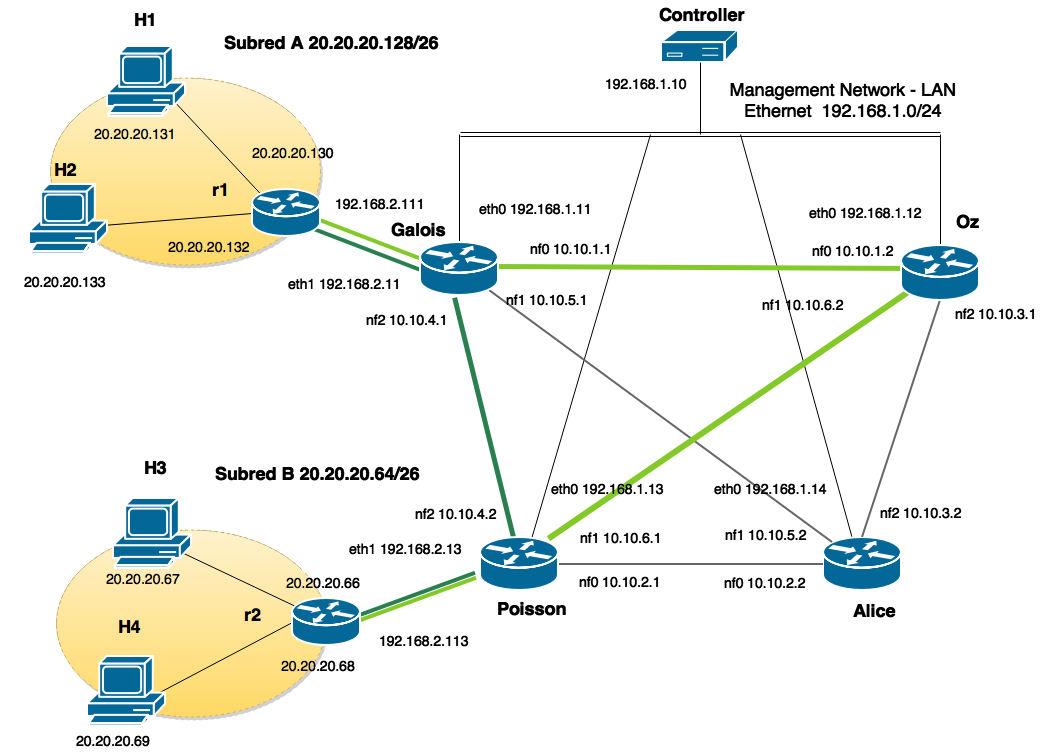
\includegraphics[width=0.85\textwidth]{CU3}
\caption[VPN de capa 2 Escenario]{VPN de capa 2 Escenario}
\label{fig:CUP3}
\end{figure}

Para generar el tr\'afico se utiliza la herramienta PacketH\cite{PacketH}, la cual permite generar paquetes asociados a diferentes protocolos desde una interfaz gr\'afica. Con esta herramienta se generan paquetes asociados a tres protocolos diferentes: ARP, IPv4 e IPv6 con tags de VLAN. En la figura \ref{fig:PaquetsSend} se muestran los paquetes generados. Por otro lado detalles m\'as t\'ecnicos como capturas tcpdump del procesamiento del tr\'afico entre otros se incluyen en el ap\'endice \ref{appendix6.4} en caso de que el lector desee profundizar en los mismos.

\begin{table}[h!]
\begin{tabular}{| l | l | l | p{4cm} | p{4cm} |}
\hline
Nombre & Ingreso & Egreso & Clasificación & Descripción \\ \hline

\crule[ForestGreen]{0.3cm}{0.3cm} S1 & Galois - eth1 & Poisson - eth1 & - & Tr\'afico de capa 2 de Subred A a Subred B \\ \hline

\crule[LimeGreen]{0.3cm}{0.3cm} S2 & Poisson - eth1 & Galois - eth1 & - & Tr\'afico de capa 2 de Subred B a Subred A \\ \hline

\end{tabular}
\vspace{0.3cm}
\caption[VPN de Capa 2, servicios creados]{VPN de Capa 2, servicios creados}
\label{table:TablaFlujos4}
\end{table}

De esta forma se verifica la capacidad de esta implementaci\'on de servicio de VPN de capa 2, para procesar tr\'afico asociado a diferentes protocolos de capas superiores definiendo un \'unico servicio. De igual forma puede verificarse la capacidad para procesar paquetes de cualquier otro protocolo de capa 3 o superiores. 

\begin{figure}[h!] 
\centering    
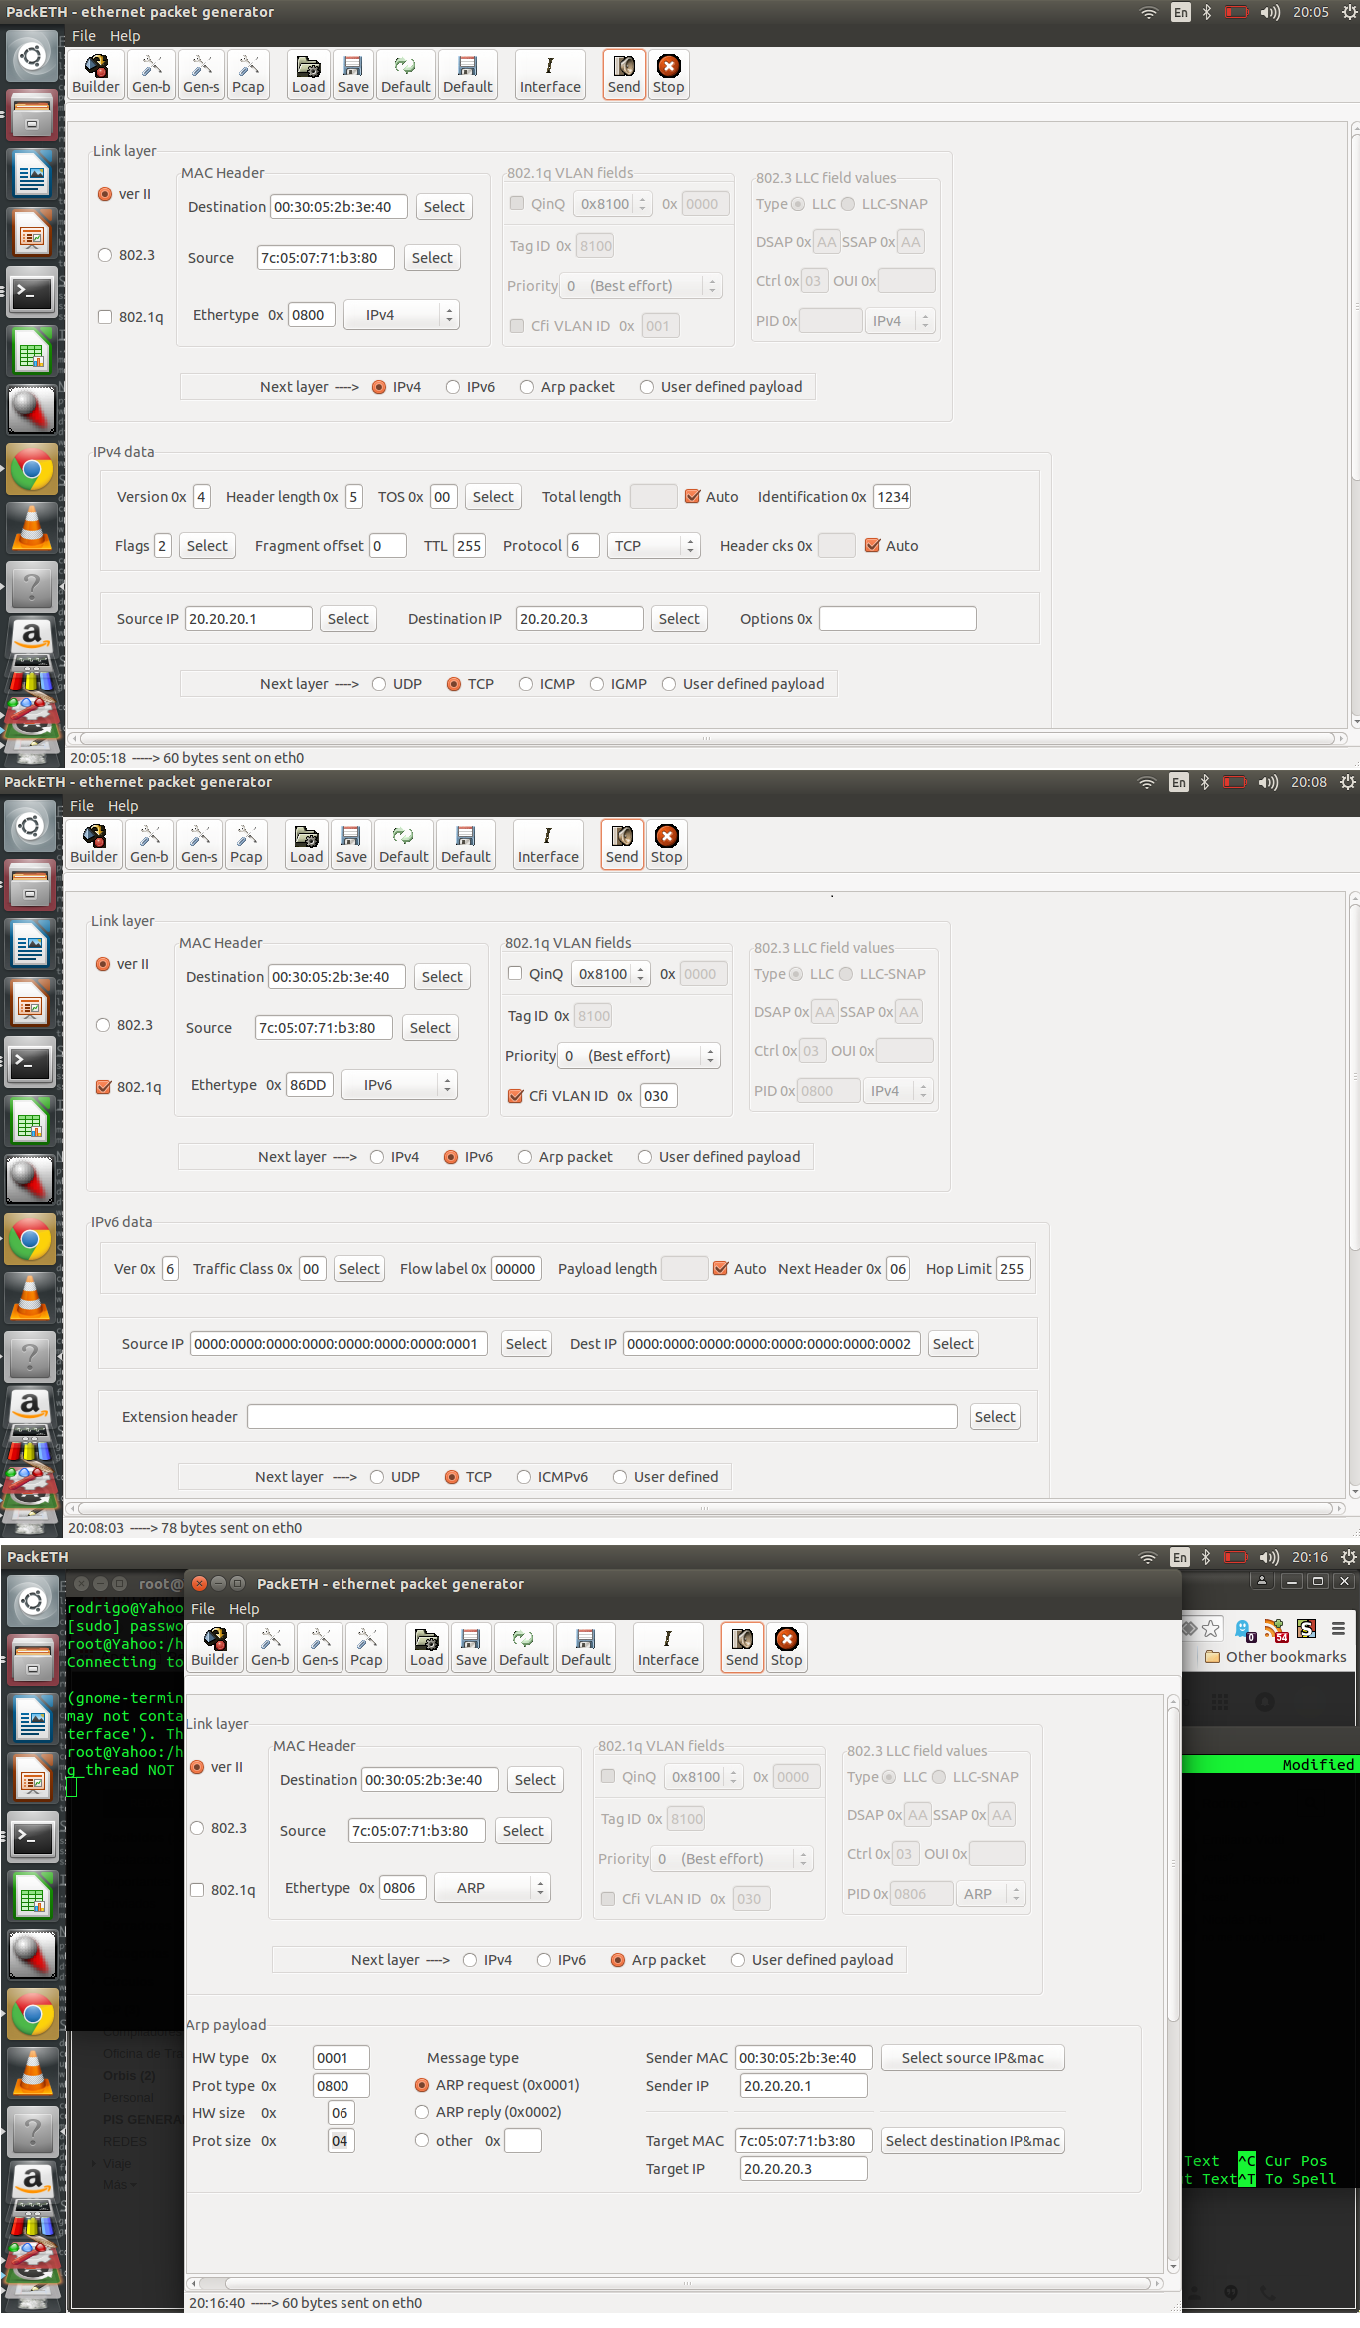
\includegraphics[width=0.75\textwidth]{Escenario3/CapMensajes}
\caption[Paquetes generados con PacketH]{Paquetes generados con PacketH}
\label{fig:PaquetsSend}
\end{figure}


